\documentclass[a4paper,12pt]{article}
\usepackage{fancyhdr}
\usepackage{graphicx}
\usepackage[export]{adjustbox}
\usepackage{caption}
\usepackage{float}
\usepackage{subcaption}
\usepackage{listings}
\usepackage{amsmath}
\usepackage{biblatex}

\addbibresource{sample.bib}

\graphicspath{ {./} }
\title{Latex cheatsheet}
\date{2021\\February}
\author{Frederik Lassen}
\pagestyle{fancy}
\fancyhf{}
\fancyfoot[R]{\thepage}
\renewcommand{\labelitemii}{$\star$}


\begin{document}
\maketitle
\thispagestyle{empty}
\clearpage
\pagenumbering{arabic}

\tableofcontents
\clearpage

\section{Introduction}
How to make danish letters
Æ Ø Å æ ø å
\section{Graphics}
\label{sec:graphics}
Let's find a picture of a cake
{
\begin{figure}[H]
	\centering
	\captionsetup{justification=centering}
	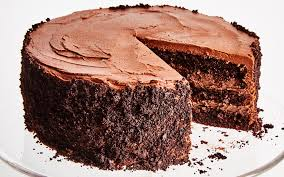
\includegraphics[scale=0.5]{cake}
	\caption{caption below, centered}
	\label{fig:cake1}
\end{figure}
}
Delicious cake. This text is not left alligned perfectly and i dont know why.
{
\begin{figure}[H]
	\centering
\begin{subfigure}{.5\textwidth}
	\centering
	\caption{caption above, left}
	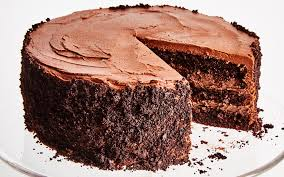
\includegraphics[width=.4\linewidth]{cake}
	\label{fig:cake2}
\end{subfigure}%
\begin{subfigure}{.5\textwidth}
	\centering
	\caption{caption above, right}
	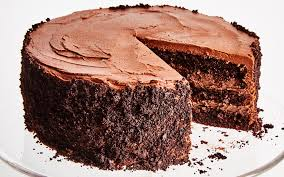
\includegraphics[width=.4\linewidth]{cake}
	\label{fig:cake3}
\end{subfigure}%
\caption{A figure with 2 subfigures}
\label{fig:double}
\end{figure}
}

\section{References}
Reference to first cake picture  ~\ref{fig:cake1} on page ~\pageref{fig:cake1} \\
Reference to second cake picture ~\ref{fig:cake2} on page ~\pageref{fig:cake2} in section ~\ref{sec:graphics} \\
Reference to third cake picture in subfigure ~\ref{fig:cake3} in  figure ~\ref{fig:double} on page ~\pageref{fig:cake3} in section ~\ref{sec:graphics}

\section{Sections}
Sections are by default numbered.
\section*{Non-numbered section}
\addcontentsline{toc}{section}{Non-numbered section}
But this one isn't
\section{Lists}
\begin{itemize}
\item this
\item is a
\item bullet point list
\end{itemize}
Break text
\begin{itemize}
\item this 
\item is a 
	\begin{itemize}
		\item stars!
		\item more stars!
	\end{itemize}
\item bullet point list
\end{itemize}
Break text
\begin{enumerate}
\item now they
\item have numbers
	\begin{enumerate}
	\item now they have letters
		\begin{enumerate}
		\item now they're roman
			\begin{enumerate}
			\item Capital letters!
			\end{enumerate}
		\end{enumerate}
	\end{enumerate}
\end{enumerate}
\clearpage
\section{Tables}

\begin{center}
\begin{tabular}{ |l|cr|| } 
 \hline
 cell1 & cell & multiple \\ 
 cell4 & columns & cell6 \\ 
 cell7 & cell8 & cell9 \\ 
 \hline
\end{tabular}
\end{center}
\begin{table}[h!]
\centering
\begin{tabular}{||c c c c||} 
 \hline
 Col1 & Col2 & Col2 & Col3 \\ [0.5ex] 
 \hline\hline
 1 & 6 & 87837 & 787 \\ 
 2 & 7 & 78 & 5415 \\
 3 & 88 & 788 & 6344 \\ [1ex] 
 \hline
\end{tabular}
\caption{Table to test captions and labels}
\label{table:1}
\end{table}
The table \ref{table:1} is an example of referenced \LaTeX elements.

\clearpage
\section{Code Listing}
\begin{verbatim}
Text enclosed inside \texttt{verbatim} environment 
is printed directly as it is
and all \LaTeX{} commands are ignored.
\end{verbatim}

Python code test

\begin{lstlisting}
import numpy as np
    
def incmatrix(genl1,genl2):
    m = len(genl1)
    n = len(genl2)
    M = None #to become the incidence matrix
    VT = np.zeros((n*m,1), int)  #dummy variable
    
    #compute the bitwise xor matrix
    M1 = bitxormatrix(genl1)
    M2 = np.triu(bitxormatrix(genl2),1) 

    for i in range(m-1):
        for j in range(i+1, m):
            [r,c] = np.where(M2 == M1[i,j])
            for k in range(len(r)):
                VT[(i)*n + r[k]] = 1;
                VT[(i)*n + c[k]] = 1;
                VT[(j)*n + r[k]] = 1;
                VT[(j)*n + c[k]] = 1;
                
                if M is None:
                    M = np.copy(VT)
                else:
                    M = np.concatenate((M, VT), 1)
                
                VT = np.zeros((n*m,1), int)
    
    return M
\end{lstlisting}

\clearpage
\section{Math equations}

 Square clamps centers and makes it look like an equation

\[ x^n + y^n = z^n \]

Dollar signs allow inline math symbols

In physics, the mass-energy equivalence is stated 
by the equation $E=mc^2$, discovered in 1905 by Albert Einstein\cite{einstein}.

You can also do this

\begin{equation}
E=mc^2
\end{equation}

Fractions can be used alongside the text, for 
example \( \frac{1}{2} \), and in a mathematical 
display style like the one below\cite{dirac}:

\[\frac{1}{2}\]

Summations

\[ \sum_{n=1}^{\infty} 2^{-n} = 1 \]

Products\cite{knuthwebsite}

Product $\prod_{i=a}^{b} f(i)$ inside text

Roots
$\sqrt{2}$

Powers $x^2$


\printbibliography
\end{document}